% Options for packages loaded elsewhere
% Options for packages loaded elsewhere
\PassOptionsToPackage{unicode}{hyperref}
\PassOptionsToPackage{hyphens}{url}
\PassOptionsToPackage{dvipsnames,svgnames,x11names}{xcolor}
%
\documentclass[
  11pt,
  a4paper,
  DIV=11,
  numbers=noendperiod]{scrartcl}
\usepackage{xcolor}
\usepackage[lmargin=2cm,rmargin=2cm,tmargin=2cm,bmargin=2cm]{geometry}
\usepackage{amsmath,amssymb}
\setcounter{secnumdepth}{-\maxdimen} % remove section numbering
\usepackage{iftex}
\ifPDFTeX
  \usepackage[T1]{fontenc}
  \usepackage[utf8]{inputenc}
  \usepackage{textcomp} % provide euro and other symbols
\else % if luatex or xetex
  \usepackage{unicode-math} % this also loads fontspec
  \defaultfontfeatures{Scale=MatchLowercase}
  \defaultfontfeatures[\rmfamily]{Ligatures=TeX,Scale=1}
\fi
\usepackage{lmodern}
\ifPDFTeX\else
  % xetex/luatex font selection
\fi
% Use upquote if available, for straight quotes in verbatim environments
\IfFileExists{upquote.sty}{\usepackage{upquote}}{}
\IfFileExists{microtype.sty}{% use microtype if available
  \usepackage[]{microtype}
  \UseMicrotypeSet[protrusion]{basicmath} % disable protrusion for tt fonts
}{}
\makeatletter
\@ifundefined{KOMAClassName}{% if non-KOMA class
  \IfFileExists{parskip.sty}{%
    \usepackage{parskip}
  }{% else
    \setlength{\parindent}{0pt}
    \setlength{\parskip}{6pt plus 2pt minus 1pt}}
}{% if KOMA class
  \KOMAoptions{parskip=half}}
\makeatother
% Make \paragraph and \subparagraph free-standing
\makeatletter
\ifx\paragraph\undefined\else
  \let\oldparagraph\paragraph
  \renewcommand{\paragraph}{
    \@ifstar
      \xxxParagraphStar
      \xxxParagraphNoStar
  }
  \newcommand{\xxxParagraphStar}[1]{\oldparagraph*{#1}\mbox{}}
  \newcommand{\xxxParagraphNoStar}[1]{\oldparagraph{#1}\mbox{}}
\fi
\ifx\subparagraph\undefined\else
  \let\oldsubparagraph\subparagraph
  \renewcommand{\subparagraph}{
    \@ifstar
      \xxxSubParagraphStar
      \xxxSubParagraphNoStar
  }
  \newcommand{\xxxSubParagraphStar}[1]{\oldsubparagraph*{#1}\mbox{}}
  \newcommand{\xxxSubParagraphNoStar}[1]{\oldsubparagraph{#1}\mbox{}}
\fi
\makeatother

\usepackage{color}
\usepackage{fancyvrb}
\newcommand{\VerbBar}{|}
\newcommand{\VERB}{\Verb[commandchars=\\\{\}]}
\DefineVerbatimEnvironment{Highlighting}{Verbatim}{commandchars=\\\{\}}
% Add ',fontsize=\small' for more characters per line
\usepackage{framed}
\definecolor{shadecolor}{RGB}{241,243,245}
\newenvironment{Shaded}{\begin{snugshade}}{\end{snugshade}}
\newcommand{\AlertTok}[1]{\textcolor[rgb]{0.68,0.00,0.00}{#1}}
\newcommand{\AnnotationTok}[1]{\textcolor[rgb]{0.37,0.37,0.37}{#1}}
\newcommand{\AttributeTok}[1]{\textcolor[rgb]{0.40,0.45,0.13}{#1}}
\newcommand{\BaseNTok}[1]{\textcolor[rgb]{0.68,0.00,0.00}{#1}}
\newcommand{\BuiltInTok}[1]{\textcolor[rgb]{0.00,0.23,0.31}{#1}}
\newcommand{\CharTok}[1]{\textcolor[rgb]{0.13,0.47,0.30}{#1}}
\newcommand{\CommentTok}[1]{\textcolor[rgb]{0.37,0.37,0.37}{#1}}
\newcommand{\CommentVarTok}[1]{\textcolor[rgb]{0.37,0.37,0.37}{\textit{#1}}}
\newcommand{\ConstantTok}[1]{\textcolor[rgb]{0.56,0.35,0.01}{#1}}
\newcommand{\ControlFlowTok}[1]{\textcolor[rgb]{0.00,0.23,0.31}{\textbf{#1}}}
\newcommand{\DataTypeTok}[1]{\textcolor[rgb]{0.68,0.00,0.00}{#1}}
\newcommand{\DecValTok}[1]{\textcolor[rgb]{0.68,0.00,0.00}{#1}}
\newcommand{\DocumentationTok}[1]{\textcolor[rgb]{0.37,0.37,0.37}{\textit{#1}}}
\newcommand{\ErrorTok}[1]{\textcolor[rgb]{0.68,0.00,0.00}{#1}}
\newcommand{\ExtensionTok}[1]{\textcolor[rgb]{0.00,0.23,0.31}{#1}}
\newcommand{\FloatTok}[1]{\textcolor[rgb]{0.68,0.00,0.00}{#1}}
\newcommand{\FunctionTok}[1]{\textcolor[rgb]{0.28,0.35,0.67}{#1}}
\newcommand{\ImportTok}[1]{\textcolor[rgb]{0.00,0.46,0.62}{#1}}
\newcommand{\InformationTok}[1]{\textcolor[rgb]{0.37,0.37,0.37}{#1}}
\newcommand{\KeywordTok}[1]{\textcolor[rgb]{0.00,0.23,0.31}{\textbf{#1}}}
\newcommand{\NormalTok}[1]{\textcolor[rgb]{0.00,0.23,0.31}{#1}}
\newcommand{\OperatorTok}[1]{\textcolor[rgb]{0.37,0.37,0.37}{#1}}
\newcommand{\OtherTok}[1]{\textcolor[rgb]{0.00,0.23,0.31}{#1}}
\newcommand{\PreprocessorTok}[1]{\textcolor[rgb]{0.68,0.00,0.00}{#1}}
\newcommand{\RegionMarkerTok}[1]{\textcolor[rgb]{0.00,0.23,0.31}{#1}}
\newcommand{\SpecialCharTok}[1]{\textcolor[rgb]{0.37,0.37,0.37}{#1}}
\newcommand{\SpecialStringTok}[1]{\textcolor[rgb]{0.13,0.47,0.30}{#1}}
\newcommand{\StringTok}[1]{\textcolor[rgb]{0.13,0.47,0.30}{#1}}
\newcommand{\VariableTok}[1]{\textcolor[rgb]{0.07,0.07,0.07}{#1}}
\newcommand{\VerbatimStringTok}[1]{\textcolor[rgb]{0.13,0.47,0.30}{#1}}
\newcommand{\WarningTok}[1]{\textcolor[rgb]{0.37,0.37,0.37}{\textit{#1}}}

\usepackage{longtable,booktabs,array}
\usepackage{calc} % for calculating minipage widths
% Correct order of tables after \paragraph or \subparagraph
\usepackage{etoolbox}
\makeatletter
\patchcmd\longtable{\par}{\if@noskipsec\mbox{}\fi\par}{}{}
\makeatother
% Allow footnotes in longtable head/foot
\IfFileExists{footnotehyper.sty}{\usepackage{footnotehyper}}{\usepackage{footnote}}
\makesavenoteenv{longtable}
\usepackage{graphicx}
\makeatletter
\newsavebox\pandoc@box
\newcommand*\pandocbounded[1]{% scales image to fit in text height/width
  \sbox\pandoc@box{#1}%
  \Gscale@div\@tempa{\textheight}{\dimexpr\ht\pandoc@box+\dp\pandoc@box\relax}%
  \Gscale@div\@tempb{\linewidth}{\wd\pandoc@box}%
  \ifdim\@tempb\p@<\@tempa\p@\let\@tempa\@tempb\fi% select the smaller of both
  \ifdim\@tempa\p@<\p@\scalebox{\@tempa}{\usebox\pandoc@box}%
  \else\usebox{\pandoc@box}%
  \fi%
}
% Set default figure placement to htbp
\def\fps@figure{htbp}
\makeatother





\setlength{\emergencystretch}{3em} % prevent overfull lines

\providecommand{\tightlist}{%
  \setlength{\itemsep}{0pt}\setlength{\parskip}{0pt}}



 


\KOMAoption{captions}{tableheading}
\makeatletter
\@ifpackageloaded{caption}{}{\usepackage{caption}}
\AtBeginDocument{%
\ifdefined\contentsname
  \renewcommand*\contentsname{Table of contents}
\else
  \newcommand\contentsname{Table of contents}
\fi
\ifdefined\listfigurename
  \renewcommand*\listfigurename{List of Figures}
\else
  \newcommand\listfigurename{List of Figures}
\fi
\ifdefined\listtablename
  \renewcommand*\listtablename{List of Tables}
\else
  \newcommand\listtablename{List of Tables}
\fi
\ifdefined\figurename
  \renewcommand*\figurename{Figure}
\else
  \newcommand\figurename{Figure}
\fi
\ifdefined\tablename
  \renewcommand*\tablename{Table}
\else
  \newcommand\tablename{Table}
\fi
}
\@ifpackageloaded{float}{}{\usepackage{float}}
\floatstyle{ruled}
\@ifundefined{c@chapter}{\newfloat{codelisting}{h}{lop}}{\newfloat{codelisting}{h}{lop}[chapter]}
\floatname{codelisting}{Listing}
\newcommand*\listoflistings{\listof{codelisting}{List of Listings}}
\makeatother
\makeatletter
\makeatother
\makeatletter
\@ifpackageloaded{caption}{}{\usepackage{caption}}
\@ifpackageloaded{subcaption}{}{\usepackage{subcaption}}
\makeatother
\usepackage{bookmark}
\IfFileExists{xurl.sty}{\usepackage{xurl}}{} % add URL line breaks if available
\urlstyle{same}
\hypersetup{
  pdftitle={Trends in University Department Preferences in Turkey (2018-2025)},
  pdfauthor={Muhammed Reha Özdemir and Yeşim Kaya},
  colorlinks=true,
  linkcolor={blue},
  filecolor={Maroon},
  citecolor={Blue},
  urlcolor={Blue},
  pdfcreator={LaTeX via pandoc}}


\title{Trends in University Department Preferences in Turkey
(2018-2025)}
\author{Muhammed Reha Özdemir and Yeşim Kaya}
\date{}
\begin{document}
\maketitle


\section{1. Project Overview and
Scope}\label{project-overview-and-scope}

\textbf{Abstract:} This study looks at how university department
preferences have changed in Turkey between 2018 and 2025 using data from
YÖK Atlas. We examined seven major field categories through admission
scores and program counts. Our results show that medicine and
dentistry/pharmacy stayed as the most competitive fields during the
whole period. Computer engineering leads among the engineering
sub-fields, with a clear upward trend toward 2025. State universities
also keep a small score advantage over private ones. A simple linear
model is applied at the end to project future score trends for computer
engineering. Overall, the results give a data-driven view of how student
preferences and higher education supply have evolved in Turkey.

This project looks at how preferences for university departments in
Turkey have shifted between 2018 and 2025. We used data from YÖK Atlas,
which is the official platform run by the Council of Higher Education.
The study tracks admission scores and program counts across seven major
field categories: engineering, medicine, law, psychology, teaching,
architecture, and dentistry/pharmacy. The main question we try to answer
is simple. Which fields are gaining or losing popularity among students,
and what might be driving these changes?

Our objectives for this study are as follows:

\begin{itemize}
\tightlist
\item
  To identify demand trends at the category level across the 2018-2025
  period
\item
  To compare engineering sub-fields, especially computer engineering
  versus civil and industrial engineering
\item
  To investigate the score gap between state and private university
  programs
\item
  To explore how programs are distributed across cities in Turkey
\item
  To build a simple trend model and estimate where admission scores
  might be heading
\end{itemize}

\section{2. Data}\label{data}

\subsection{2.1 Data Sources}\label{data-sources}

We combined three data sources to cover the full 2018-2025 period. The
first one is the \texttt{thestats} R package developed by Mustafa Cavus
and Olgun Aydin. This package provides structured YÖK Atlas data for the
years 2018 to 2020. It is very convenient for the early years, but its
coverage stops at 2020. To fill the 2021 gap, we used a third-party
dataset from GitHub (MorphaxTheDeveloper), which was compiled from YÖK
Atlas records for that year. For the more recent years between 2022 and
2025, we pulled data directly from the YÖK Atlas JSON API using the
\texttt{httr2} package in R. Among the three sources, the API data is
the most reliable since it comes from the official system. The
third-party 2021 dataset needed extra verification during preprocessing.

References: YÖK Atlas (\url{https://yokatlas.yok.gov.tr/}), thestats
package (\url{https://github.com/analyticsresearchlab/thestats}),
MorphaxTheDeveloper dataset
(\url{https://github.com/MorphaxTheDeveloper/yokatlas-dataset-2025})

\subsection{2.2 Preprocessing}\label{preprocessing}

The three sources use slightly different column names and encoding
conventions. We merged them into a single table and standardized
department names by matching Turkish and English variants. University
type labels (\texttt{unitur}) were also unified. Finally, we added a
\texttt{bolum\_grubu} column to group programs into broader
sub-categories for easier comparison.

\begin{Shaded}
\begin{Highlighting}[]
\CommentTok{\# Read the combined dataset}
\NormalTok{df }\OtherTok{\textless{}{-}} \FunctionTok{fread}\NormalTok{(}\StringTok{"yokatlas\_FINAL\_CLEAN.csv"}\NormalTok{, }\AttributeTok{encoding =} \StringTok{"UTF{-}8"}\NormalTok{)}

\CommentTok{\# Convert to tibble for tidyverse compatibility}
\NormalTok{df }\OtherTok{\textless{}{-}} \FunctionTok{as\_tibble}\NormalTok{(df)}

\CommentTok{\# Quick structure check}
\FunctionTok{cat}\NormalTok{(}\StringTok{"Dataset dimensions:"}\NormalTok{, }\FunctionTok{nrow}\NormalTok{(df), }\StringTok{"rows x"}\NormalTok{, }\FunctionTok{ncol}\NormalTok{(df), }\StringTok{"columns}\SpecialCharTok{\textbackslash{}n}\StringTok{"}\NormalTok{)}
\end{Highlighting}
\end{Shaded}

\begin{verbatim}
Dataset dimensions: 75145 rows x 11 columns
\end{verbatim}

\begin{Shaded}
\begin{Highlighting}[]
\FunctionTok{cat}\NormalTok{(}\StringTok{"Years covered:"}\NormalTok{, }\FunctionTok{paste}\NormalTok{(}\FunctionTok{sort}\NormalTok{(}\FunctionTok{unique}\NormalTok{(df}\SpecialCharTok{$}\NormalTok{year)), }\AttributeTok{collapse =} \StringTok{", "}\NormalTok{), }\StringTok{"}\SpecialCharTok{\textbackslash{}n}\StringTok{"}\NormalTok{)}
\end{Highlighting}
\end{Shaded}

\begin{verbatim}
Years covered: 2018, 2019, 2020, 2021, 2022, 2023, 2024, 2025 
\end{verbatim}

\begin{Shaded}
\begin{Highlighting}[]
\FunctionTok{cat}\NormalTok{(}\StringTok{"Categories:"}\NormalTok{, }\FunctionTok{paste}\NormalTok{(}\FunctionTok{sort}\NormalTok{(}\FunctionTok{unique}\NormalTok{(df}\SpecialCharTok{$}\NormalTok{kategori)), }\AttributeTok{collapse =} \StringTok{", "}\NormalTok{), }\StringTok{"}\SpecialCharTok{\textbackslash{}n}\StringTok{"}\NormalTok{)}
\end{Highlighting}
\end{Shaded}

\begin{verbatim}
Categories: Diger, Dis_Hekimligi_Eczacilik, Hukuk, Mimarlik, Muhendislik, Ogretmenlik, Psikoloji, Tip 
\end{verbatim}

\begin{Shaded}
\begin{Highlighting}[]
\CommentTok{\# Save as .RData for reproducibility}
\FunctionTok{save}\NormalTok{(df, }\AttributeTok{file =} \StringTok{"data.RData"}\NormalTok{)}
\end{Highlighting}
\end{Shaded}

The processed dataset is stored in \texttt{.RData} format and can be
accessed \href{data.RData}{here}.

\subsection{2.3 Data Overview}\label{data-overview}

The dataset contains the following key columns:

\begin{longtable}[]{@{}
  >{\raggedright\arraybackslash}p{(\linewidth - 2\tabcolsep) * \real{0.2222}}
  >{\raggedright\arraybackslash}p{(\linewidth - 2\tabcolsep) * \real{0.7778}}@{}}
\toprule\noalign{}
\begin{minipage}[b]{\linewidth}\raggedright
Column
\end{minipage} & \begin{minipage}[b]{\linewidth}\raggedright
Description
\end{minipage} \\
\midrule\noalign{}
\endhead
\bottomrule\noalign{}
\endlastfoot
\texttt{year} & Academic year of admission \\
\texttt{kategori} & Field category (e.g., Muhendislik, Tip) \\
\texttt{bolum\_grubu} & Sub-grouping of programs (engineering sub-fields
+ main fields) \\
\texttt{il} & City where the university is located \\
\texttt{unitur} & University type: DEVLET (state) or VAKIF (private) \\
\texttt{puan} & Minimum admission score for the program \\
\texttt{sira} & Admission rank corresponding to the minimum score \\
\texttt{kontenjan} & Total quota (capacity) of the program \\
\texttt{yerlesen} & Number of students actually enrolled \\
\end{longtable}

\begin{Shaded}
\begin{Highlighting}[]
\CommentTok{\# Programs per year}
\NormalTok{df }\SpecialCharTok{|\textgreater{}}
  \FunctionTok{group\_by}\NormalTok{(year) }\SpecialCharTok{|\textgreater{}}
  \FunctionTok{summarise}\NormalTok{(}\AttributeTok{n\_programs =} \FunctionTok{n}\NormalTok{(),}
            \AttributeTok{avg\_puan =} \FunctionTok{round}\NormalTok{(}\FunctionTok{mean}\NormalTok{(puan, }\AttributeTok{na.rm =} \ConstantTok{TRUE}\NormalTok{), }\DecValTok{1}\NormalTok{),}
            \AttributeTok{avg\_sira =} \FunctionTok{round}\NormalTok{(}\FunctionTok{mean}\NormalTok{(sira, }\AttributeTok{na.rm =} \ConstantTok{TRUE}\NormalTok{), }\DecValTok{0}\NormalTok{)) }\SpecialCharTok{|\textgreater{}}
  \FunctionTok{print}\NormalTok{()}
\end{Highlighting}
\end{Shaded}

\begin{verbatim}
# A tibble: 8 x 4
   year n_programs avg_puan avg_sira
  <int>      <int>    <dbl>    <dbl>
1  2018       5935     323.   198128
2  2019       6764     324.   239592
3  2020       9571     318.   312161
4  2021      18357     175    329515
5  2022       8354     284    359386
6  2023       8927     272.   382464
7  2024       9640     243.   391498
8  2025       7597     334.   336911
\end{verbatim}

\begin{Shaded}
\begin{Highlighting}[]
\CommentTok{\# Programs per category}
\NormalTok{df }\SpecialCharTok{|\textgreater{}}
  \FunctionTok{filter}\NormalTok{(kategori }\SpecialCharTok{!=} \StringTok{"Diger"}\NormalTok{) }\SpecialCharTok{|\textgreater{}}
  \FunctionTok{group\_by}\NormalTok{(kategori) }\SpecialCharTok{|\textgreater{}}
  \FunctionTok{summarise}\NormalTok{(}\AttributeTok{n\_programs =} \FunctionTok{n}\NormalTok{(),}
            \AttributeTok{avg\_puan =} \FunctionTok{round}\NormalTok{(}\FunctionTok{mean}\NormalTok{(puan, }\AttributeTok{na.rm =} \ConstantTok{TRUE}\NormalTok{), }\DecValTok{1}\NormalTok{)) }\SpecialCharTok{|\textgreater{}}
  \FunctionTok{arrange}\NormalTok{(}\FunctionTok{desc}\NormalTok{(avg\_puan)) }\SpecialCharTok{|\textgreater{}}
  \FunctionTok{print}\NormalTok{()}
\end{Highlighting}
\end{Shaded}

\begin{verbatim}
# A tibble: 7 x 3
  kategori                n_programs avg_puan
  <chr>                        <int>    <dbl>
1 Tip                           1323     433.
2 Dis_Hekimligi_Eczacilik       1673     396.
3 Hukuk                         1178     350.
4 Ogretmenlik                   4204     323.
5 Psikoloji                     2801     306.
6 Muhendislik                  13495     291.
7 Mimarlik                      3106     266.
\end{verbatim}

The dataset covers eight academic years and contains records from all
seven field categories. Medicine has the highest average admission score
at 433, followed by dentistry/pharmacy at 396. Architecture sits at the
bottom with 266. Engineering has the largest number of programs by far,
with over 13,000 records across all years. It averages around 291, which
reflects the wide range of programs it includes. The 2021 row shows an
unusually high program count of 18,357. This is likely an artifact of
how the third-party data source for that year was structured, rather
than a real spike in offerings.

\section{3. Analysis}\label{analysis}

\subsection{3.1 Exploratory Data
Analysis}\label{exploratory-data-analysis}

\begin{Shaded}
\begin{Highlighting}[]
\NormalTok{df }\SpecialCharTok{|\textgreater{}}
  \FunctionTok{filter}\NormalTok{(kategori }\SpecialCharTok{!=} \StringTok{"Diger"}\NormalTok{, year }\SpecialCharTok{==} \DecValTok{2024}\NormalTok{) }\SpecialCharTok{|\textgreater{}}
  \FunctionTok{ggplot}\NormalTok{(}\FunctionTok{aes}\NormalTok{(}\AttributeTok{x =}\NormalTok{ kategori, }\AttributeTok{y =}\NormalTok{ puan, }\AttributeTok{fill =}\NormalTok{ kategori)) }\SpecialCharTok{+}
  \FunctionTok{geom\_boxplot}\NormalTok{(}\AttributeTok{show.legend =} \ConstantTok{FALSE}\NormalTok{) }\SpecialCharTok{+}
  \FunctionTok{labs}\NormalTok{(}\AttributeTok{title =} \StringTok{"Score Distribution by Category (2024)"}\NormalTok{,}
       \AttributeTok{x =} \ConstantTok{NULL}\NormalTok{, }\AttributeTok{y =} \StringTok{"Minimum Admission Score"}\NormalTok{) }\SpecialCharTok{+}
  \FunctionTok{theme\_minimal}\NormalTok{() }\SpecialCharTok{+}
  \FunctionTok{theme}\NormalTok{(}\AttributeTok{axis.text.x =} \FunctionTok{element\_text}\NormalTok{(}\AttributeTok{angle =} \DecValTok{25}\NormalTok{, }\AttributeTok{hjust =} \DecValTok{1}\NormalTok{))}
\end{Highlighting}
\end{Shaded}

\begin{figure}[H]

\centering{

\pandocbounded{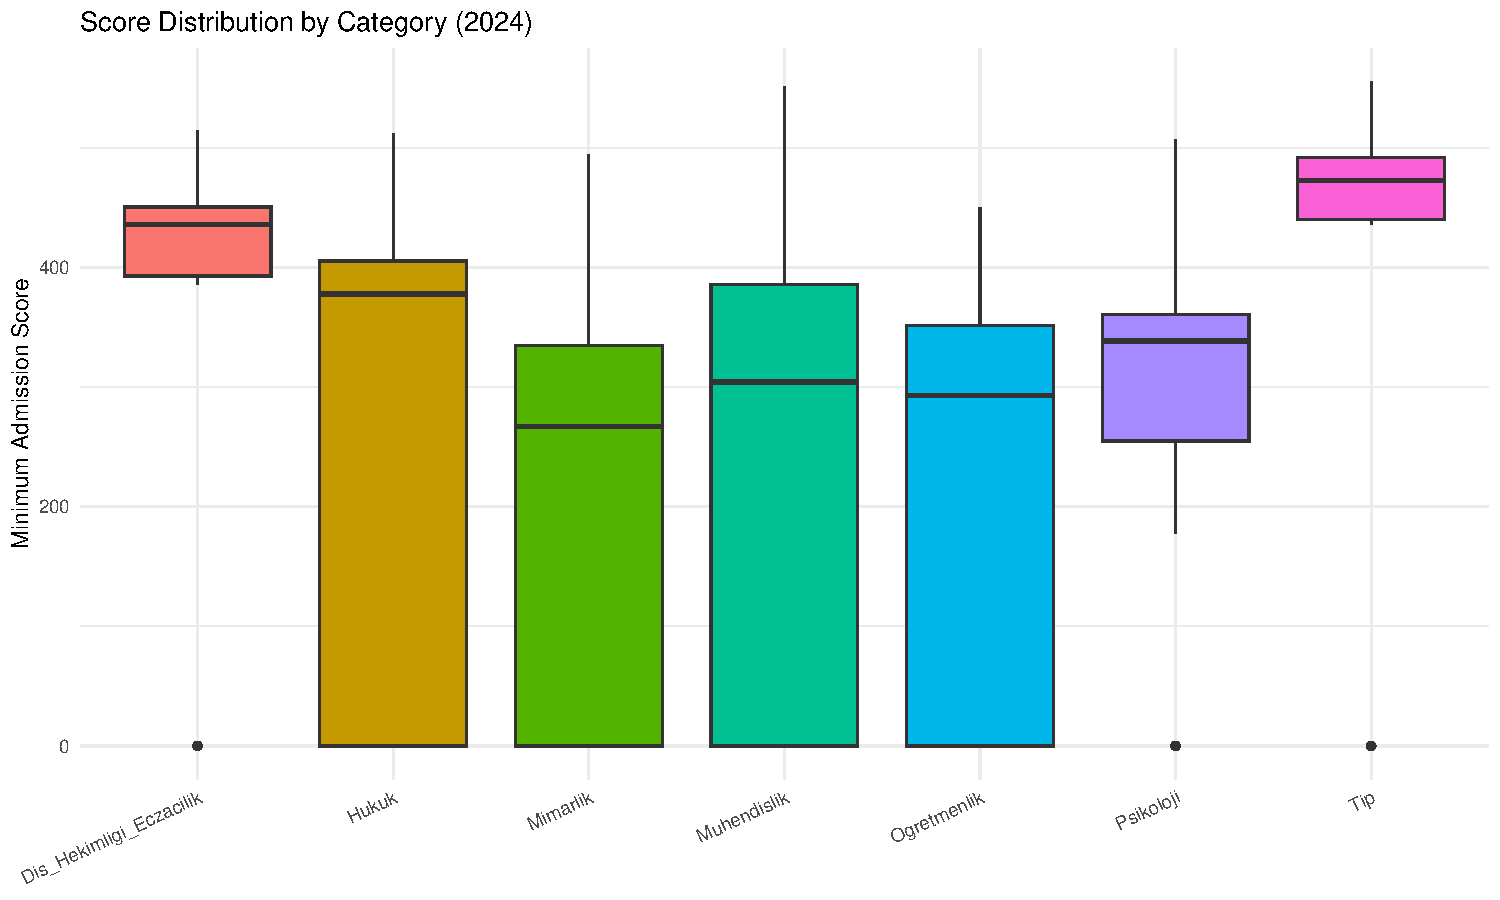
\includegraphics[keepaspectratio]{project_files/figure-pdf/fig-eda-distribution-1.pdf}}

}

\caption{\label{fig-eda-distribution}Minimum admission score
distribution across field categories in 2024.}

\end{figure}%

Looking at Figure~\ref{fig-eda-distribution}, the 2024 score
distributions show a lot of variation both across and within categories.
Medicine and dentistry/pharmacy have the highest and most compact
distributions. This means most programs in these fields require similar
high scores. Law and engineering show wider spreads. Engineering covers
a very broad range, from around 0 to well above 400. This points to the
existence of very selective programs and much lower-threshold ones
within the same category. Psychology's interquartile range sits mostly
between 250 and 375, with a few outliers near zero that are likely
low-quota private programs.

\begin{Shaded}
\begin{Highlighting}[]
\NormalTok{df }\SpecialCharTok{|\textgreater{}}
  \FunctionTok{filter}\NormalTok{(year }\SpecialCharTok{==} \DecValTok{2024}\NormalTok{, }\SpecialCharTok{!}\FunctionTok{is.na}\NormalTok{(puan), puan }\SpecialCharTok{\textgreater{}} \DecValTok{0}\NormalTok{) }\SpecialCharTok{|\textgreater{}}
  \FunctionTok{ggplot}\NormalTok{(}\FunctionTok{aes}\NormalTok{(}\AttributeTok{x =}\NormalTok{ puan)) }\SpecialCharTok{+}
  \FunctionTok{geom\_histogram}\NormalTok{(}\AttributeTok{bins =} \DecValTok{40}\NormalTok{, }\AttributeTok{fill =} \StringTok{"\#2E86AB"}\NormalTok{, }\AttributeTok{color =} \StringTok{"white"}\NormalTok{) }\SpecialCharTok{+}
  \FunctionTok{labs}\NormalTok{(}\AttributeTok{title =} \StringTok{"Distribution of Minimum Admission Scores (2024)"}\NormalTok{,}
       \AttributeTok{x =} \StringTok{"Minimum Admission Score"}\NormalTok{, }\AttributeTok{y =} \StringTok{"Count"}\NormalTok{) }\SpecialCharTok{+}
  \FunctionTok{theme\_minimal}\NormalTok{()}
\end{Highlighting}
\end{Shaded}

\begin{figure}[H]

\centering{

\pandocbounded{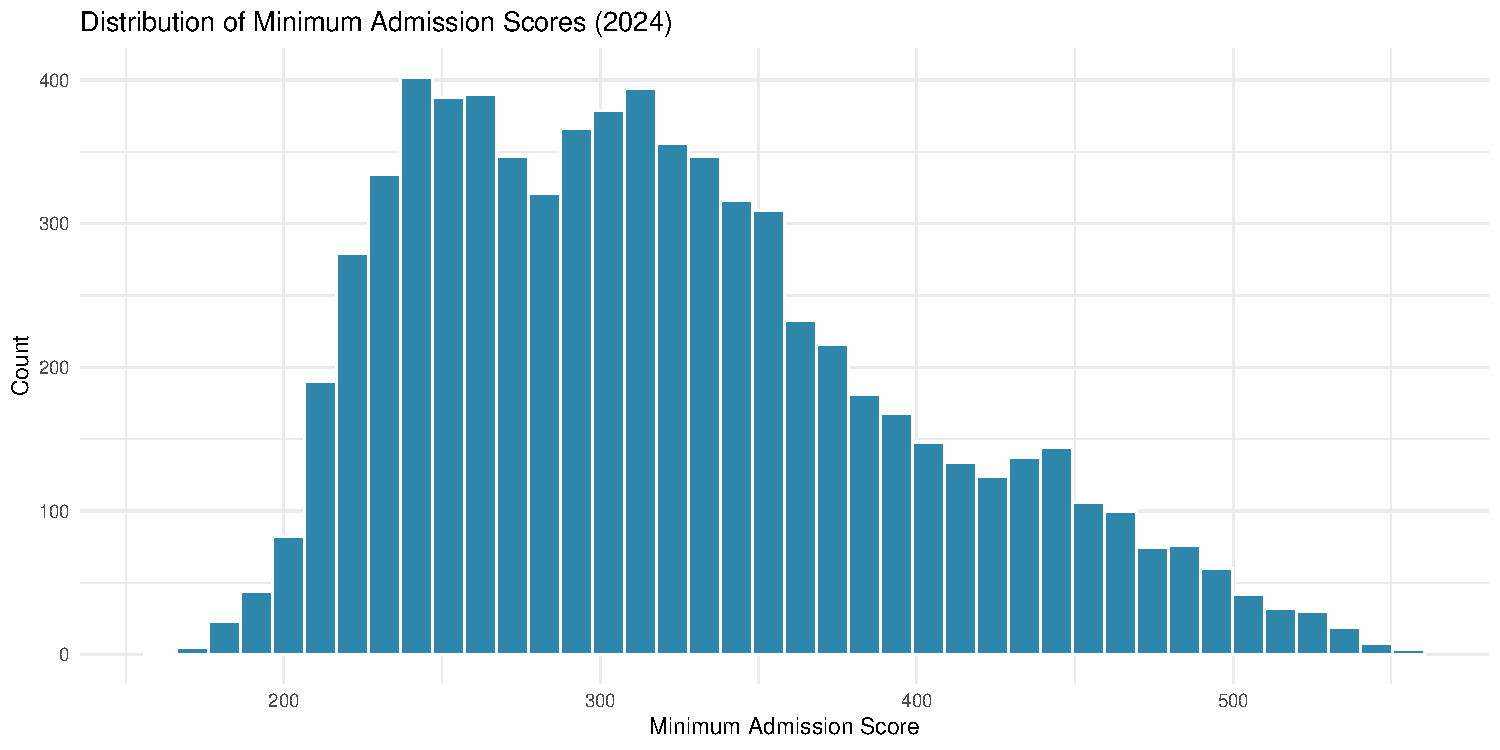
\includegraphics[keepaspectratio]{project_files/figure-pdf/fig-eda-histogram-1.pdf}}

}

\caption{\label{fig-eda-histogram}Histogram of minimum admission scores
across all programs in 2024.}

\end{figure}%

The overall distribution of admission scores in 2024 is roughly
bell-shaped, as Figure~\ref{fig-eda-histogram} shows. The highest
concentration of programs falls between 250 and 350 points. There is
also a secondary cluster near the lower end of the scale. These are
mostly programs that did not fully fill their quotas or have very low
demand.

\begin{Shaded}
\begin{Highlighting}[]
\NormalTok{df }\SpecialCharTok{|\textgreater{}}
  \FunctionTok{summarise}\NormalTok{(}
    \AttributeTok{kontenjan\_na =} \FunctionTok{sum}\NormalTok{(}\FunctionTok{is.na}\NormalTok{(kontenjan)),}
    \AttributeTok{yerlesen\_na  =} \FunctionTok{sum}\NormalTok{(}\FunctionTok{is.na}\NormalTok{(yerlesen)),}
    \AttributeTok{puan\_na      =} \FunctionTok{sum}\NormalTok{(}\FunctionTok{is.na}\NormalTok{(puan)),}
    \AttributeTok{sira\_na      =} \FunctionTok{sum}\NormalTok{(}\FunctionTok{is.na}\NormalTok{(sira))}
\NormalTok{  ) }\SpecialCharTok{|\textgreater{}}
  \FunctionTok{print}\NormalTok{()}
\end{Highlighting}
\end{Shaded}

\begin{verbatim}
# A tibble: 1 x 4
  kontenjan_na yerlesen_na puan_na sira_na
         <int>       <int>   <int>   <int>
1        28148        4452       0    5357
\end{verbatim}

Missing values are mostly in the \texttt{yerlesen} (enrolled students)
and \texttt{sira} (rank) columns. This is expected since not all
programs fill their quotas every year. Also, rank data is not always
published for very low-scoring entries. The \texttt{puan} column is our
primary variable, and it has a relatively small number of missing
entries. We excluded these from calculations using
\texttt{na.rm\ =\ TRUE}.

\begin{table}

\caption{\label{tbl-summary-stats}}

\centering{

\begin{Shaded}
\begin{Highlighting}[]
\NormalTok{df }\SpecialCharTok{|\textgreater{}}
  \FunctionTok{filter}\NormalTok{(year }\SpecialCharTok{==} \DecValTok{2024}\NormalTok{, kategori }\SpecialCharTok{!=} \StringTok{"Diger"}\NormalTok{, }\SpecialCharTok{!}\FunctionTok{is.na}\NormalTok{(puan)) }\SpecialCharTok{|\textgreater{}}
  \FunctionTok{group\_by}\NormalTok{(kategori) }\SpecialCharTok{|\textgreater{}}
  \FunctionTok{summarise}\NormalTok{(}
    \AttributeTok{n =} \FunctionTok{n}\NormalTok{(),}
    \AttributeTok{mean\_puan =} \FunctionTok{round}\NormalTok{(}\FunctionTok{mean}\NormalTok{(puan), }\DecValTok{1}\NormalTok{),}
    \AttributeTok{median\_puan =} \FunctionTok{round}\NormalTok{(}\FunctionTok{median}\NormalTok{(puan), }\DecValTok{1}\NormalTok{),}
    \AttributeTok{sd\_puan =} \FunctionTok{round}\NormalTok{(}\FunctionTok{sd}\NormalTok{(puan), }\DecValTok{1}\NormalTok{),}
    \AttributeTok{iqr\_puan =} \FunctionTok{round}\NormalTok{(}\FunctionTok{IQR}\NormalTok{(puan), }\DecValTok{1}\NormalTok{)}
\NormalTok{  ) }\SpecialCharTok{|\textgreater{}}
  \FunctionTok{arrange}\NormalTok{(}\FunctionTok{desc}\NormalTok{(median\_puan)) }\SpecialCharTok{|\textgreater{}}
  \FunctionTok{print}\NormalTok{()}
\end{Highlighting}
\end{Shaded}

\begin{verbatim}
# A tibble: 7 x 6
  kategori                    n mean_puan median_puan sd_puan iqr_puan
  <chr>                   <int>     <dbl>       <dbl>   <dbl>    <dbl>
1 Tip                       241      382.        473.    197.     52.1
2 Dis_Hekimligi_Eczacilik   307      336.        436.    189.     57.6
3 Hukuk                     177      296.        378.    176.    405. 
4 Psikoloji                 480      290.        338.    119.    106. 
5 Muhendislik              2255      230.        304.    188.    385. 
6 Ogretmenlik               354      176.        293.    176.    351. 
7 Mimarlik                  474      227.        267     145.    335. 
\end{verbatim}

}

\end{table}%

The summary table above gives us a clearer picture. One thing that
stands out is the big gap between mean and median values in every
category. For medicine, the mean is 381 while the median is 472. For
engineering, it is 230 versus 304. This happens because the mean is
pulled down by programs that did not fill or scored very low. The median
is a much more reliable indicator of the ``typical'' program in each
category. The standard deviation is also high across the board, which
confirms the wide internal spread we already saw in the boxplot.

\begin{table}

\caption{\label{tbl-correlations}}

\centering{

\begin{Shaded}
\begin{Highlighting}[]
\CommentTok{\# Pearson correlation matrix for numerical variables}
\NormalTok{df }\SpecialCharTok{|\textgreater{}}
  \FunctionTok{select}\NormalTok{(kontenjan, yerlesen, puan, sira) }\SpecialCharTok{|\textgreater{}}
  \FunctionTok{na.omit}\NormalTok{() }\SpecialCharTok{|\textgreater{}}
  \FunctionTok{cor}\NormalTok{() }\SpecialCharTok{|\textgreater{}}
  \FunctionTok{round}\NormalTok{(}\DecValTok{3}\NormalTok{) }\SpecialCharTok{|\textgreater{}}
  \FunctionTok{print}\NormalTok{()}
\end{Highlighting}
\end{Shaded}

\begin{verbatim}
          kontenjan yerlesen   puan   sira
kontenjan     1.000    0.974  0.006  0.045
yerlesen      0.974    1.000  0.072  0.074
puan          0.006    0.072  1.000 -0.134
sira          0.045    0.074 -0.134  1.000
\end{verbatim}

}

\end{table}%

The correlation matrix gives a few interesting results. First, the
correlation between \texttt{kontenjan} (quota) and \texttt{yerlesen}
(enrolled students) is 0.97, which is almost perfect. This tells us that
most programs in Turkey fill very close to their full capacity. Second,
\texttt{puan} and \texttt{sira} show a weak negative correlation of
about -0.13. This makes sense (higher score = lower rank number), but
the relationship is weaker than expected, probably because the data
mixes very different score types (SAY, EA) across categories. Third,
\texttt{puan} and \texttt{kontenjan} have a correlation near zero. So
the size of a program is not really tied to how selective it is. A
small, low-demand program can have a low score just as easily as a large
one.

\subsection{3.2 Category Trend Analysis}\label{category-trend-analysis}

\begin{Shaded}
\begin{Highlighting}[]
\CommentTok{\# Average minimum score by category over years}
\NormalTok{category\_trend }\OtherTok{\textless{}{-}}\NormalTok{ df }\SpecialCharTok{|\textgreater{}}
  \FunctionTok{filter}\NormalTok{(kategori }\SpecialCharTok{!=} \StringTok{"Diger"}\NormalTok{) }\SpecialCharTok{|\textgreater{}}
  \FunctionTok{group\_by}\NormalTok{(year, kategori) }\SpecialCharTok{|\textgreater{}}
  \FunctionTok{summarise}\NormalTok{(}\AttributeTok{avg\_puan =} \FunctionTok{mean}\NormalTok{(puan, }\AttributeTok{na.rm =} \ConstantTok{TRUE}\NormalTok{), }\AttributeTok{.groups =} \StringTok{"drop"}\NormalTok{)}

\FunctionTok{ggplot}\NormalTok{(category\_trend, }\FunctionTok{aes}\NormalTok{(}\AttributeTok{x =}\NormalTok{ year, }\AttributeTok{y =}\NormalTok{ avg\_puan, }\AttributeTok{color =}\NormalTok{ kategori)) }\SpecialCharTok{+}
  \FunctionTok{geom\_line}\NormalTok{(}\AttributeTok{linewidth =} \FloatTok{1.1}\NormalTok{) }\SpecialCharTok{+}
  \FunctionTok{geom\_point}\NormalTok{(}\AttributeTok{size =} \DecValTok{2}\NormalTok{) }\SpecialCharTok{+}
  \FunctionTok{scale\_x\_continuous}\NormalTok{(}\AttributeTok{breaks =} \DecValTok{2018}\SpecialCharTok{:}\DecValTok{2025}\NormalTok{) }\SpecialCharTok{+}
  \FunctionTok{labs}\NormalTok{(}\AttributeTok{title =} \StringTok{"Average Minimum Admission Score by Category (2018{-}2025)"}\NormalTok{,}
       \AttributeTok{x =} \StringTok{"Year"}\NormalTok{, }\AttributeTok{y =} \StringTok{"Average Min Score"}\NormalTok{, }\AttributeTok{color =} \StringTok{"Category"}\NormalTok{) }\SpecialCharTok{+}
  \FunctionTok{theme\_minimal}\NormalTok{()}
\end{Highlighting}
\end{Shaded}

\begin{figure}[H]

\centering{

\pandocbounded{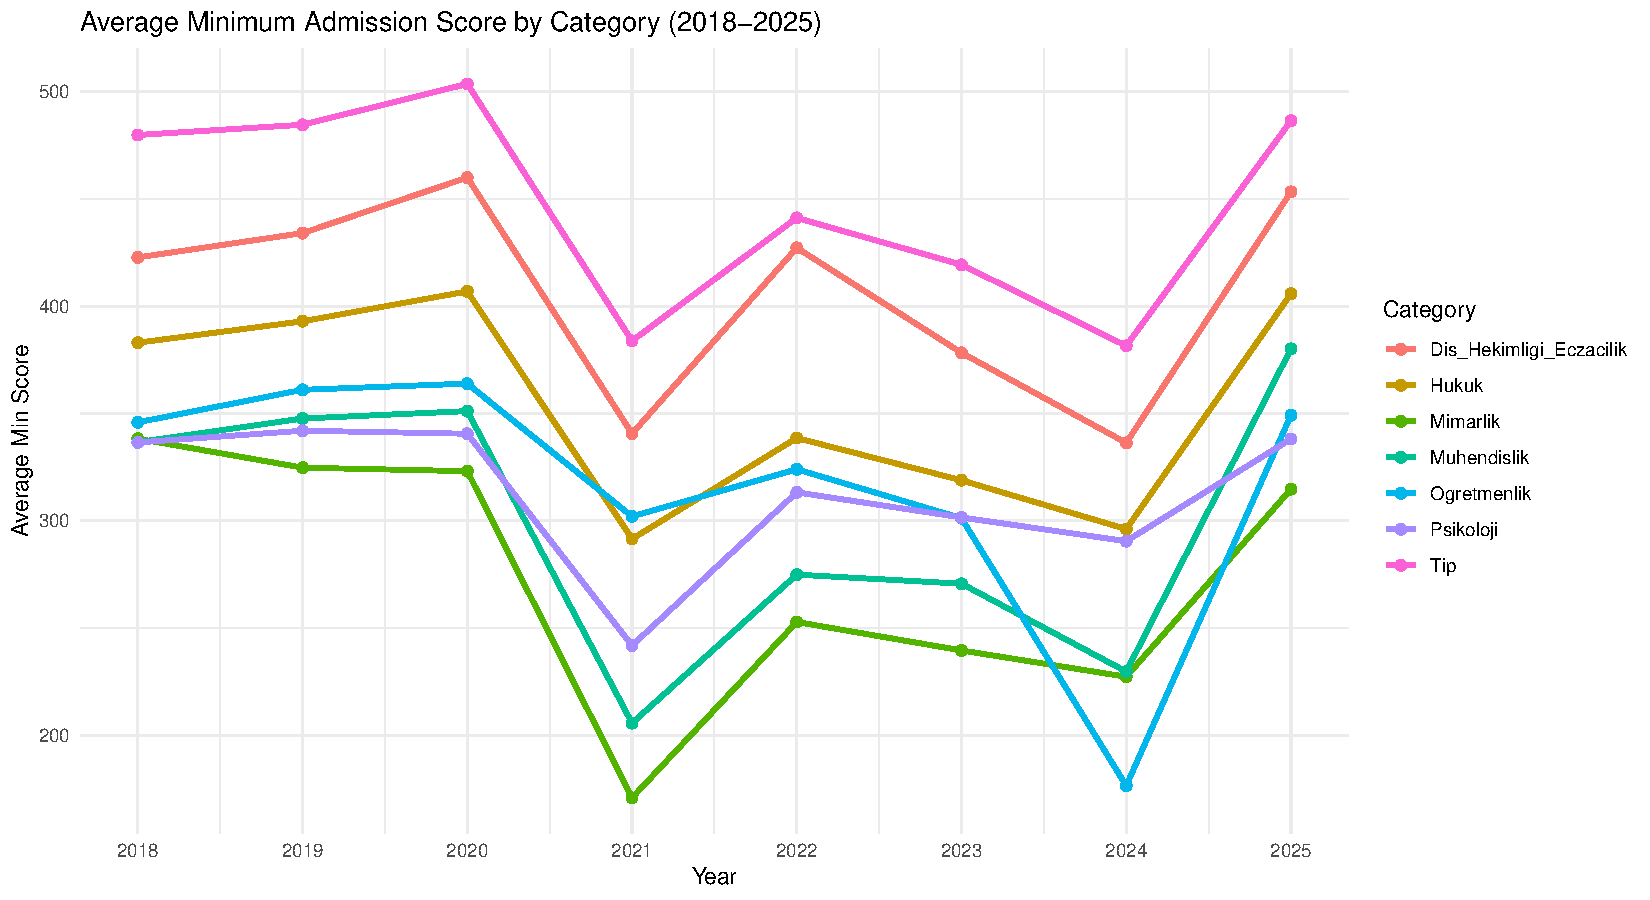
\includegraphics[keepaspectratio]{project_files/figure-pdf/fig-category-trend-puan-1.pdf}}

}

\caption{\label{fig-category-trend-puan}Average minimum admission score
by field category from 2018 to 2025.}

\end{figure}%

The most striking feature of Figure~\ref{fig-category-trend-puan} is the
sharp drop across all categories in 2021, followed by a partial recovery
in 2022. This pattern probably comes from a data source change for 2021
rather than a real-year effect, so it should be read with caution. If we
put that aside, medicine and dentistry/pharmacy have held the highest
scores during the whole period, and both show an upward push toward
2025. Law recovered strongly after 2022 and is trending upward.
Engineering and architecture have stayed relatively flat. Psychology and
teaching remain in the lower range with no clear directional movement.

\begin{Shaded}
\begin{Highlighting}[]
\CommentTok{\# Program count trend}
\NormalTok{program\_count }\OtherTok{\textless{}{-}}\NormalTok{ df }\SpecialCharTok{|\textgreater{}}
  \FunctionTok{filter}\NormalTok{(kategori }\SpecialCharTok{!=} \StringTok{"Diger"}\NormalTok{) }\SpecialCharTok{|\textgreater{}}
  \FunctionTok{group\_by}\NormalTok{(year, kategori) }\SpecialCharTok{|\textgreater{}}
  \FunctionTok{summarise}\NormalTok{(}\AttributeTok{n =} \FunctionTok{n}\NormalTok{(), }\AttributeTok{.groups =} \StringTok{"drop"}\NormalTok{)}

\FunctionTok{ggplot}\NormalTok{(program\_count, }\FunctionTok{aes}\NormalTok{(}\AttributeTok{x =}\NormalTok{ year, }\AttributeTok{y =}\NormalTok{ n, }\AttributeTok{color =}\NormalTok{ kategori)) }\SpecialCharTok{+}
  \FunctionTok{geom\_line}\NormalTok{(}\AttributeTok{linewidth =} \FloatTok{1.1}\NormalTok{) }\SpecialCharTok{+}
  \FunctionTok{geom\_point}\NormalTok{(}\AttributeTok{size =} \DecValTok{2}\NormalTok{) }\SpecialCharTok{+}
  \FunctionTok{scale\_x\_continuous}\NormalTok{(}\AttributeTok{breaks =} \DecValTok{2018}\SpecialCharTok{:}\DecValTok{2025}\NormalTok{) }\SpecialCharTok{+}
  \FunctionTok{labs}\NormalTok{(}\AttributeTok{title =} \StringTok{"Number of Programs by Category (2018{-}2025)"}\NormalTok{,}
       \AttributeTok{x =} \StringTok{"Year"}\NormalTok{, }\AttributeTok{y =} \StringTok{"Number of Programs"}\NormalTok{, }\AttributeTok{color =} \StringTok{"Category"}\NormalTok{) }\SpecialCharTok{+}
  \FunctionTok{theme\_minimal}\NormalTok{()}
\end{Highlighting}
\end{Shaded}

\begin{figure}[H]

\centering{

\pandocbounded{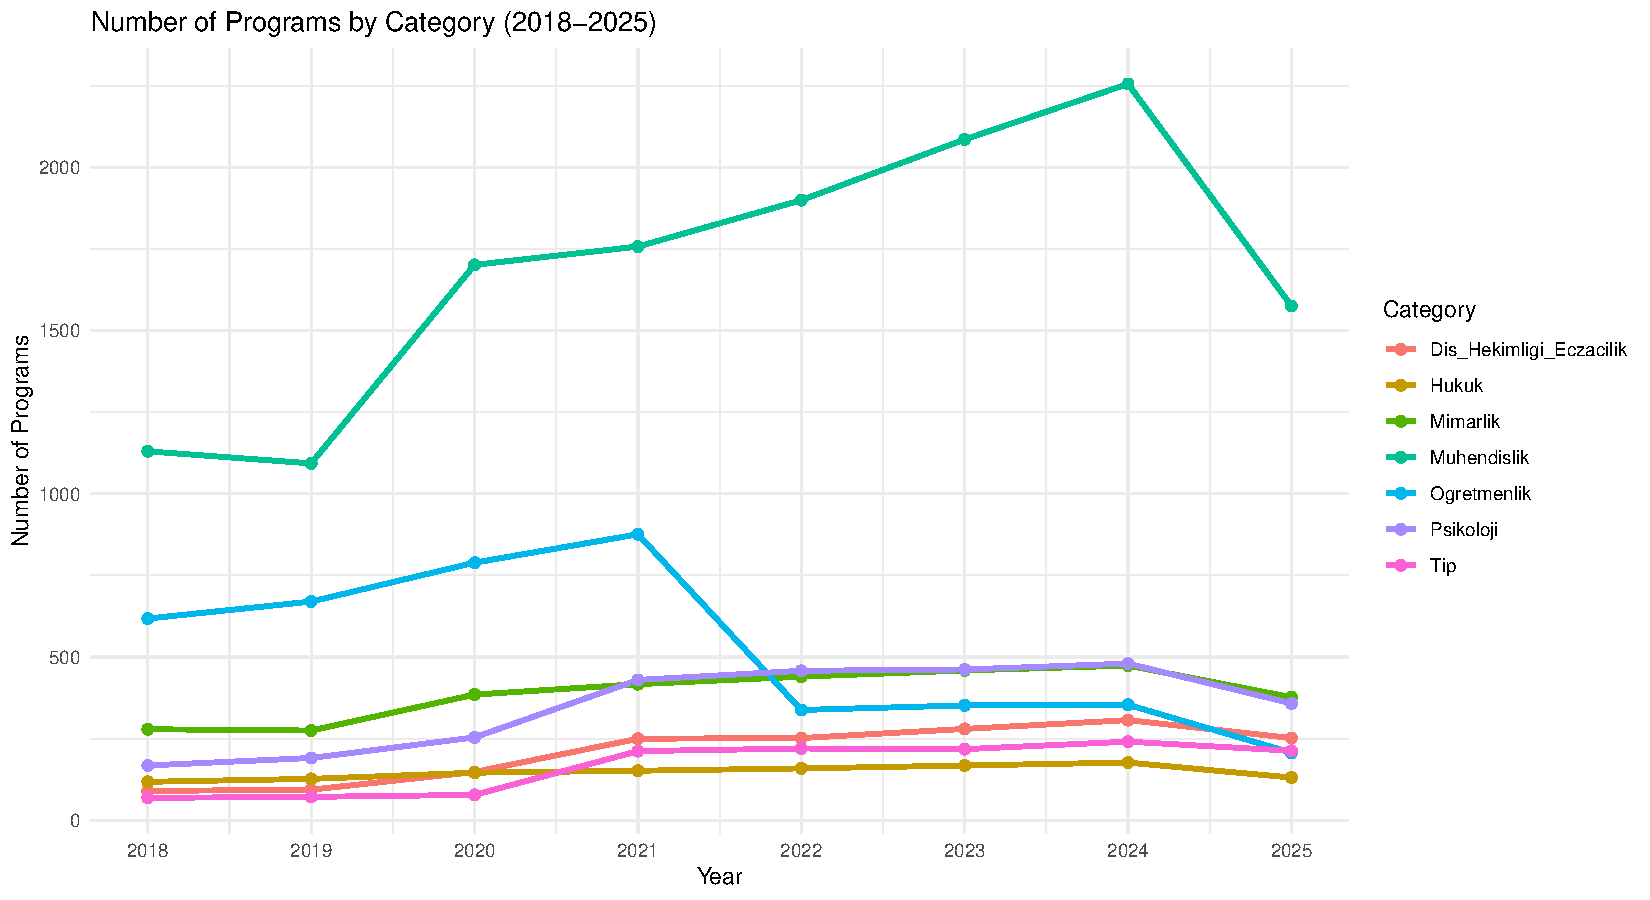
\includegraphics[keepaspectratio]{project_files/figure-pdf/fig-category-trend-count-1.pdf}}

}

\caption{\label{fig-category-trend-count}Number of programs per field
category from 2018 to 2025.}

\end{figure}%

In Figure~\ref{fig-category-trend-count}, engineering dominates the
program count chart throughout the entire period. It reached a peak of
around 2,300 programs in 2024 before dropping in 2025. Teaching is the
second largest category, but it shows a sharp decline after 2021. This
is possibly due to quota reductions by the government. Psychology has
grown modestly but steadily. It went from near the bottom of the chart
in 2018 to clearly separating itself from the smaller categories by
2024. Dentistry/pharmacy and medicine remain flat and low in count,
which is consistent with the controlled and limited capacity of those
fields.

\subsection{3.3 Engineering Sub-field
Analysis}\label{engineering-sub-field-analysis}

\begin{Shaded}
\begin{Highlighting}[]
\CommentTok{\# Top 6 engineering sub{-}fields by program count}
\NormalTok{top\_eng }\OtherTok{\textless{}{-}}\NormalTok{ df }\SpecialCharTok{|\textgreater{}}
  \FunctionTok{filter}\NormalTok{(kategori }\SpecialCharTok{==} \StringTok{"Muhendislik"}\NormalTok{,}
\NormalTok{         bolum\_grubu }\SpecialCharTok{!=} \StringTok{"Diger Muhendislik"}\NormalTok{) }\SpecialCharTok{|\textgreater{}}
  \FunctionTok{group\_by}\NormalTok{(bolum\_grubu) }\SpecialCharTok{|\textgreater{}}
  \FunctionTok{summarise}\NormalTok{(}\AttributeTok{n =} \FunctionTok{n}\NormalTok{()) }\SpecialCharTok{|\textgreater{}}
  \FunctionTok{arrange}\NormalTok{(}\FunctionTok{desc}\NormalTok{(n)) }\SpecialCharTok{|\textgreater{}}
  \FunctionTok{head}\NormalTok{(}\DecValTok{6}\NormalTok{) }\SpecialCharTok{|\textgreater{}}
  \FunctionTok{pull}\NormalTok{(bolum\_grubu)}

\CommentTok{\# Score trend for top sub{-}fields}
\NormalTok{eng\_trend }\OtherTok{\textless{}{-}}\NormalTok{ df }\SpecialCharTok{|\textgreater{}}
  \FunctionTok{filter}\NormalTok{(bolum\_grubu }\SpecialCharTok{\%in\%}\NormalTok{ top\_eng) }\SpecialCharTok{|\textgreater{}}
  \FunctionTok{group\_by}\NormalTok{(year, bolum\_grubu) }\SpecialCharTok{|\textgreater{}}
  \FunctionTok{summarise}\NormalTok{(}\AttributeTok{avg\_puan =} \FunctionTok{mean}\NormalTok{(puan, }\AttributeTok{na.rm =} \ConstantTok{TRUE}\NormalTok{), }\AttributeTok{.groups =} \StringTok{"drop"}\NormalTok{)}

\FunctionTok{ggplot}\NormalTok{(eng\_trend, }\FunctionTok{aes}\NormalTok{(}\AttributeTok{x =}\NormalTok{ year, }\AttributeTok{y =}\NormalTok{ avg\_puan, }\AttributeTok{color =}\NormalTok{ bolum\_grubu)) }\SpecialCharTok{+}
  \FunctionTok{geom\_line}\NormalTok{(}\AttributeTok{linewidth =} \FloatTok{1.1}\NormalTok{) }\SpecialCharTok{+}
  \FunctionTok{geom\_point}\NormalTok{(}\AttributeTok{size =} \DecValTok{2}\NormalTok{) }\SpecialCharTok{+}
  \FunctionTok{scale\_x\_continuous}\NormalTok{(}\AttributeTok{breaks =} \DecValTok{2018}\SpecialCharTok{:}\DecValTok{2025}\NormalTok{) }\SpecialCharTok{+}
  \FunctionTok{labs}\NormalTok{(}\AttributeTok{title =} \StringTok{"Top 6 Engineering Sub{-}fields: Admission Score Trend"}\NormalTok{,}
       \AttributeTok{x =} \StringTok{"Year"}\NormalTok{, }\AttributeTok{y =} \StringTok{"Average Min Score"}\NormalTok{, }\AttributeTok{color =} \StringTok{"Sub{-}field"}\NormalTok{) }\SpecialCharTok{+}
  \FunctionTok{theme\_minimal}\NormalTok{()}
\end{Highlighting}
\end{Shaded}

\begin{figure}[H]

\centering{

\pandocbounded{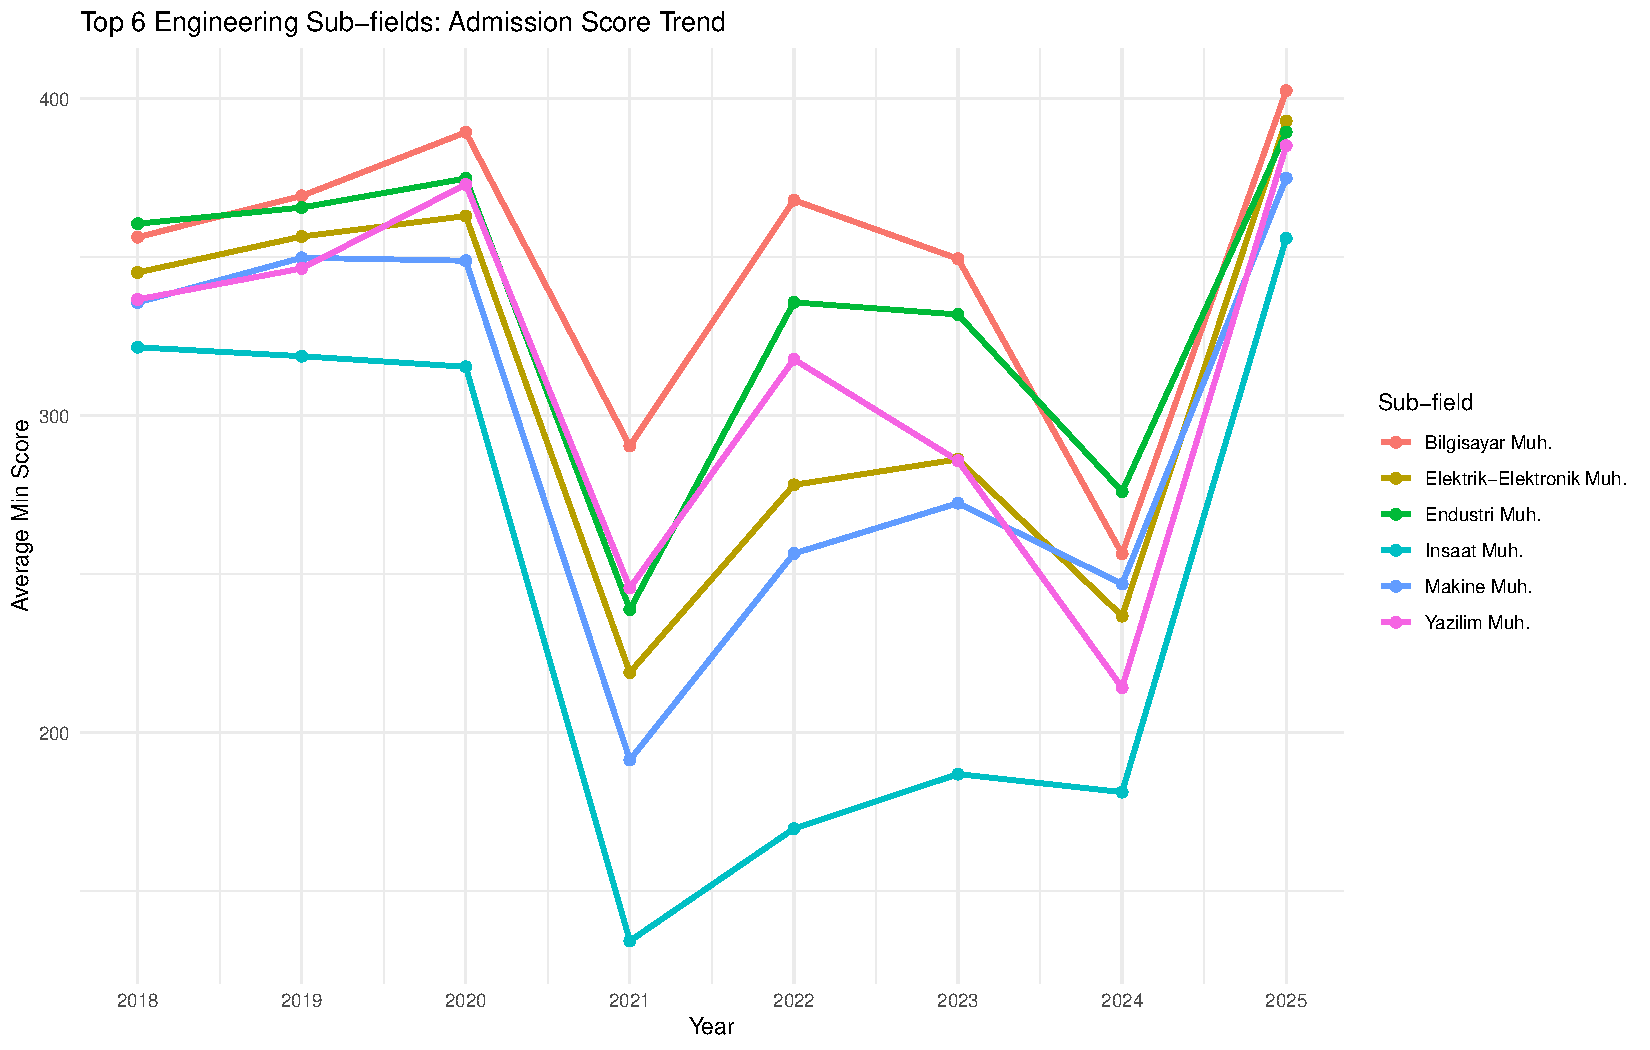
\includegraphics[keepaspectratio]{project_files/figure-pdf/fig-eng-subfield-trend-1.pdf}}

}

\caption{\label{fig-eng-subfield-trend}Average minimum admission score
trend for the top 6 engineering sub-fields.}

\end{figure}%

Among the six sub-fields in Figure~\ref{fig-eng-subfield-trend},
computer engineering has kept the highest average scores for most of the
period and shows a strong recovery toward 2025, reaching around 400.
Software engineering follows a similar upward trajectory in recent
years. Industrial engineering and electrical-electronics engineering
have tracked each other closely throughout, sitting in the mid-range.
Civil engineering stays at the bottom of the group and shows the widest
dip in 2021. It seems to be the most sensitive sub-field to whatever
data issue affected that year. The overall pattern across all sub-fields
is a convergence upward in 2025, which may reflect a real increase in
competition across engineering as a whole.

\begin{Shaded}
\begin{Highlighting}[]
\NormalTok{df }\SpecialCharTok{|\textgreater{}}
  \FunctionTok{filter}\NormalTok{(bolum\_grubu }\SpecialCharTok{\%in\%}\NormalTok{ top\_eng, year }\SpecialCharTok{\textgreater{}=} \DecValTok{2022}\NormalTok{) }\SpecialCharTok{|\textgreater{}}
  \FunctionTok{ggplot}\NormalTok{(}\FunctionTok{aes}\NormalTok{(}\AttributeTok{x =}\NormalTok{ puan, }\AttributeTok{fill =}\NormalTok{ bolum\_grubu)) }\SpecialCharTok{+}
  \FunctionTok{geom\_histogram}\NormalTok{(}\AttributeTok{bins =} \DecValTok{25}\NormalTok{, }\AttributeTok{show.legend =} \ConstantTok{FALSE}\NormalTok{, }\AttributeTok{color =} \StringTok{"white"}\NormalTok{) }\SpecialCharTok{+}
  \FunctionTok{facet\_wrap}\NormalTok{(}\SpecialCharTok{\textasciitilde{}}\NormalTok{bolum\_grubu, }\AttributeTok{scales =} \StringTok{"free\_y"}\NormalTok{) }\SpecialCharTok{+}
  \FunctionTok{labs}\NormalTok{(}\AttributeTok{title =} \StringTok{"Score Distribution of Top Engineering Sub{-}fields (2022{-}2025)"}\NormalTok{,}
       \AttributeTok{x =} \StringTok{"Minimum Admission Score"}\NormalTok{, }\AttributeTok{y =} \StringTok{"Count"}\NormalTok{) }\SpecialCharTok{+}
  \FunctionTok{theme\_minimal}\NormalTok{()}
\end{Highlighting}
\end{Shaded}

\begin{figure}[H]

\centering{

\pandocbounded{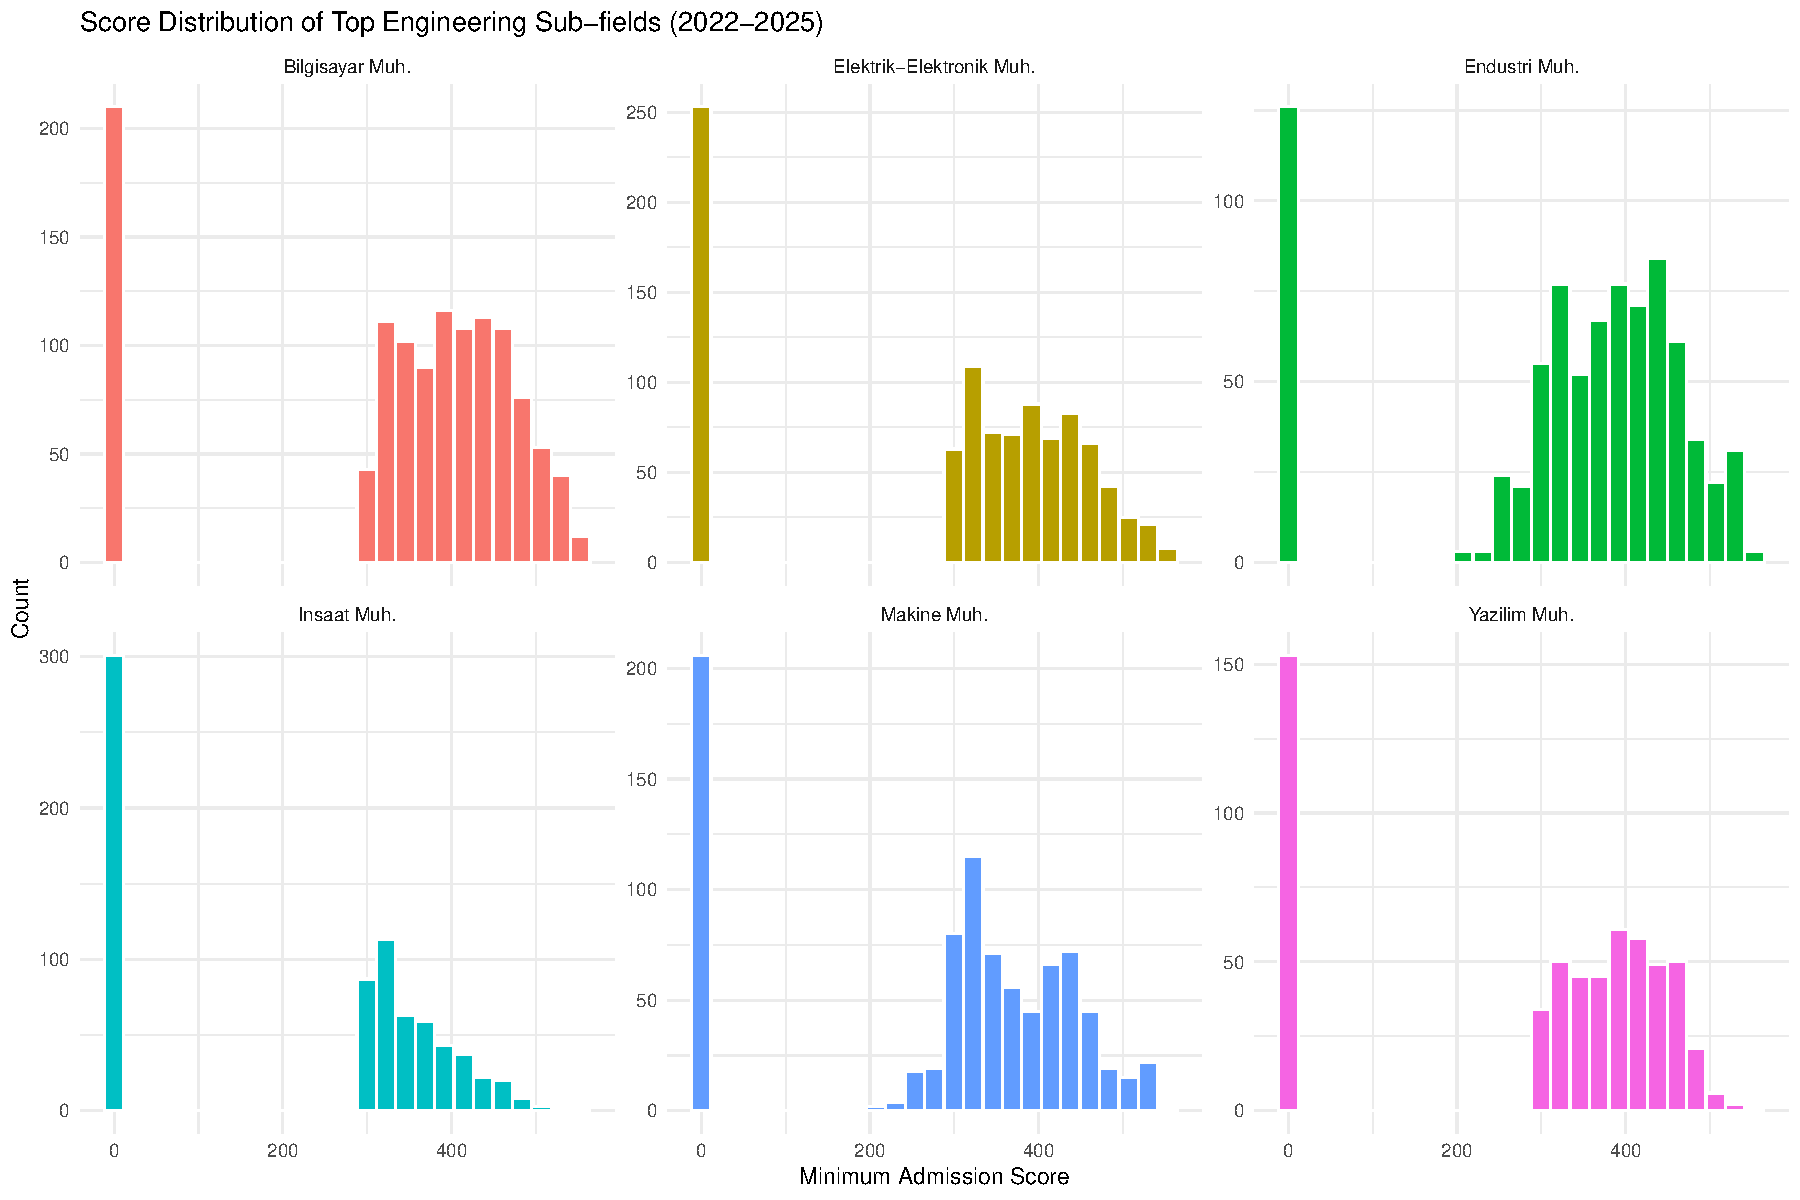
\includegraphics[keepaspectratio]{project_files/figure-pdf/fig-eng-facet-1.pdf}}

}

\caption{\label{fig-eng-facet}Score distribution panels for the top 6
engineering sub-fields (2022-2025).}

\end{figure}%

Figure~\ref{fig-eng-facet} highlights the differences between sub-fields
more clearly. Computer engineering has a wider distribution that is
shifted toward higher scores. Civil engineering programs, on the other
hand, are clustered at the lower end. This confirms that the demand gap
between sub-fields is not only about averages. It extends across the
entire score range.

\begin{Shaded}
\begin{Highlighting}[]
\NormalTok{df }\SpecialCharTok{|\textgreater{}}
  \FunctionTok{filter}\NormalTok{(kategori }\SpecialCharTok{==} \StringTok{"Muhendislik"}\NormalTok{,}
\NormalTok{         unitur }\SpecialCharTok{\%in\%} \FunctionTok{c}\NormalTok{(}\StringTok{"DEVLET"}\NormalTok{, }\StringTok{"VAKIF"}\NormalTok{),}
\NormalTok{         year }\SpecialCharTok{==} \DecValTok{2024}\NormalTok{) }\SpecialCharTok{|\textgreater{}}
  \FunctionTok{ggplot}\NormalTok{(}\FunctionTok{aes}\NormalTok{(}\AttributeTok{x =}\NormalTok{ unitur, }\AttributeTok{y =}\NormalTok{ puan, }\AttributeTok{fill =}\NormalTok{ unitur)) }\SpecialCharTok{+}
  \FunctionTok{geom\_boxplot}\NormalTok{(}\AttributeTok{show.legend =} \ConstantTok{FALSE}\NormalTok{) }\SpecialCharTok{+}
  \FunctionTok{scale\_fill\_manual}\NormalTok{(}\AttributeTok{values =} \FunctionTok{c}\NormalTok{(}\StringTok{"DEVLET"} \OtherTok{=} \StringTok{"\#2E86AB"}\NormalTok{, }\StringTok{"VAKIF"} \OtherTok{=} \StringTok{"\#F39C12"}\NormalTok{)) }\SpecialCharTok{+}
  \FunctionTok{labs}\NormalTok{(}\AttributeTok{title =} \StringTok{"State vs Private: Engineering Score Distribution (2024)"}\NormalTok{,}
       \AttributeTok{x =} \ConstantTok{NULL}\NormalTok{, }\AttributeTok{y =} \StringTok{"Minimum Admission Score"}\NormalTok{) }\SpecialCharTok{+}
  \FunctionTok{theme\_minimal}\NormalTok{()}
\end{Highlighting}
\end{Shaded}

\begin{figure}[H]

\centering{

\pandocbounded{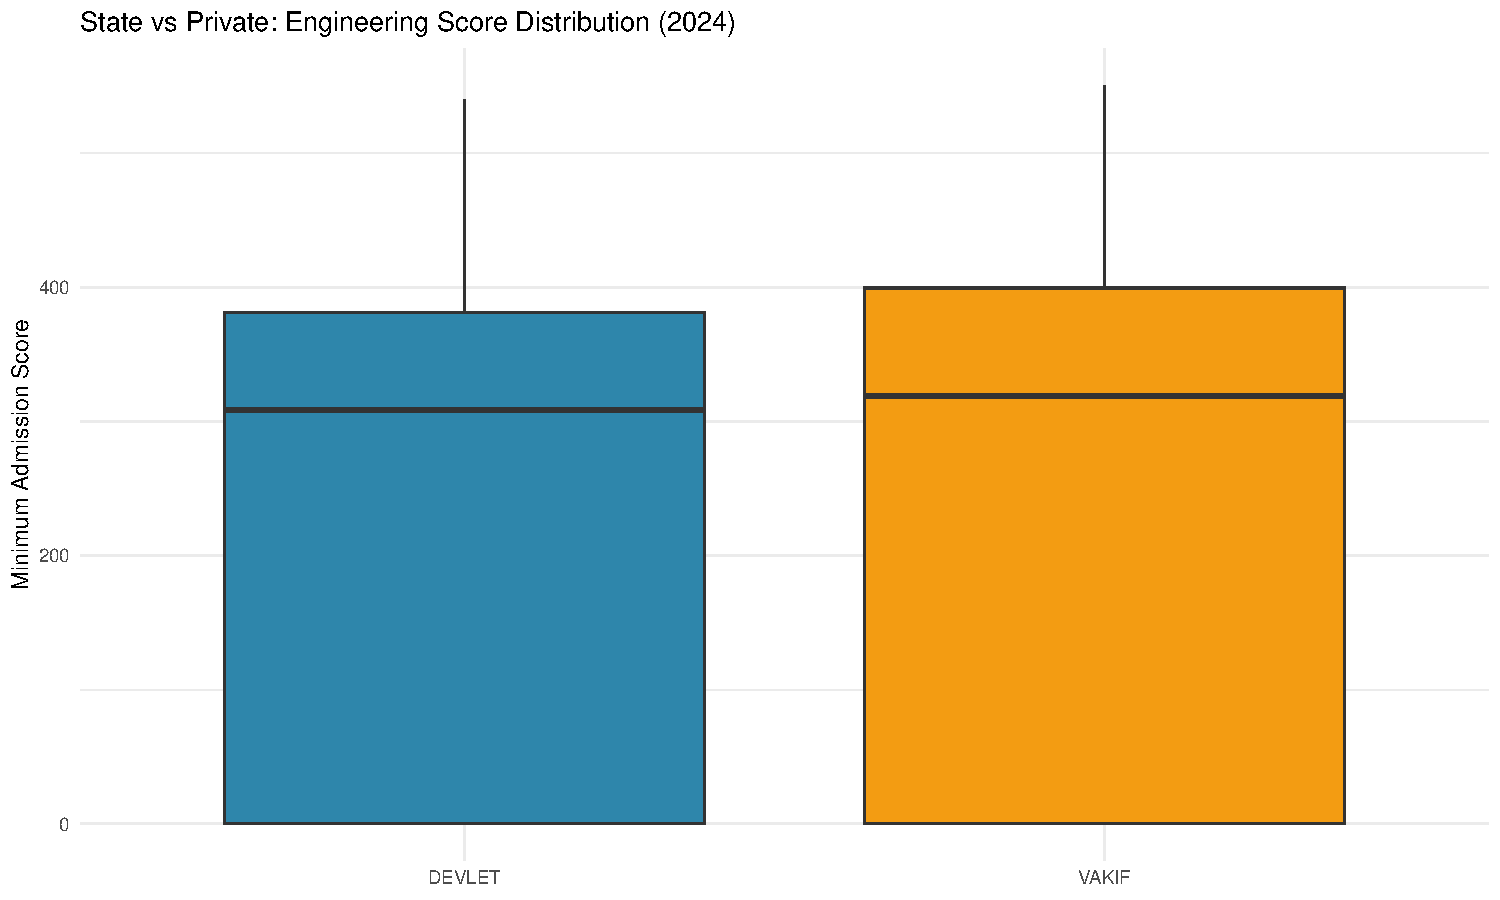
\includegraphics[keepaspectratio]{project_files/figure-pdf/fig-eng-state-private-1.pdf}}

}

\caption{\label{fig-eng-state-private}Minimum admission score
distribution for state and private engineering programs in 2024.}

\end{figure}%

Contrary to what we might expect, Figure~\ref{fig-eng-state-private}
shows that the score distributions for state and private engineering
programs in 2024 are quite similar in terms of median (both sit around
280-290). The main difference is in the spread. Private university
programs show a wider interquartile range and a longer lower tail. This
means there are more private programs with very low admission scores
pulling their distribution down. State programs also have very low
outliers, but their overall box is slightly more compact. The difference
is real but not as dramatic as we initially thought.

\subsection{3.4 Regional Analysis}\label{regional-analysis}

\begin{Shaded}
\begin{Highlighting}[]
\NormalTok{top\_cities }\OtherTok{\textless{}{-}}\NormalTok{ df }\SpecialCharTok{|\textgreater{}}
  \FunctionTok{filter}\NormalTok{(}\SpecialCharTok{!}\FunctionTok{is.na}\NormalTok{(il), il }\SpecialCharTok{!=} \StringTok{""}\NormalTok{, year }\SpecialCharTok{==} \DecValTok{2024}\NormalTok{, kategori }\SpecialCharTok{!=} \StringTok{"Diger"}\NormalTok{) }\SpecialCharTok{|\textgreater{}}
  \FunctionTok{group\_by}\NormalTok{(il) }\SpecialCharTok{|\textgreater{}}
  \FunctionTok{summarise}\NormalTok{(}\AttributeTok{n\_programs =} \FunctionTok{n}\NormalTok{(),}
            \AttributeTok{avg\_puan =} \FunctionTok{round}\NormalTok{(}\FunctionTok{mean}\NormalTok{(puan, }\AttributeTok{na.rm =} \ConstantTok{TRUE}\NormalTok{), }\DecValTok{1}\NormalTok{)) }\SpecialCharTok{|\textgreater{}}
  \FunctionTok{arrange}\NormalTok{(}\FunctionTok{desc}\NormalTok{(n\_programs)) }\SpecialCharTok{|\textgreater{}}
  \FunctionTok{head}\NormalTok{(}\DecValTok{10}\NormalTok{)}

\FunctionTok{ggplot}\NormalTok{(top\_cities, }\FunctionTok{aes}\NormalTok{(}\AttributeTok{x =} \FunctionTok{reorder}\NormalTok{(il, n\_programs), }\AttributeTok{y =}\NormalTok{ n\_programs)) }\SpecialCharTok{+}
  \FunctionTok{geom\_col}\NormalTok{(}\AttributeTok{fill =} \StringTok{"\#2E86AB"}\NormalTok{) }\SpecialCharTok{+}
  \FunctionTok{coord\_flip}\NormalTok{() }\SpecialCharTok{+}
  \FunctionTok{labs}\NormalTok{(}\AttributeTok{title =} \StringTok{"Top 10 Cities by Number of Programs (2024)"}\NormalTok{,}
       \AttributeTok{x =} \ConstantTok{NULL}\NormalTok{, }\AttributeTok{y =} \StringTok{"Number of Programs"}\NormalTok{) }\SpecialCharTok{+}
  \FunctionTok{theme\_minimal}\NormalTok{()}
\end{Highlighting}
\end{Shaded}

\begin{figure}[H]

\centering{

\pandocbounded{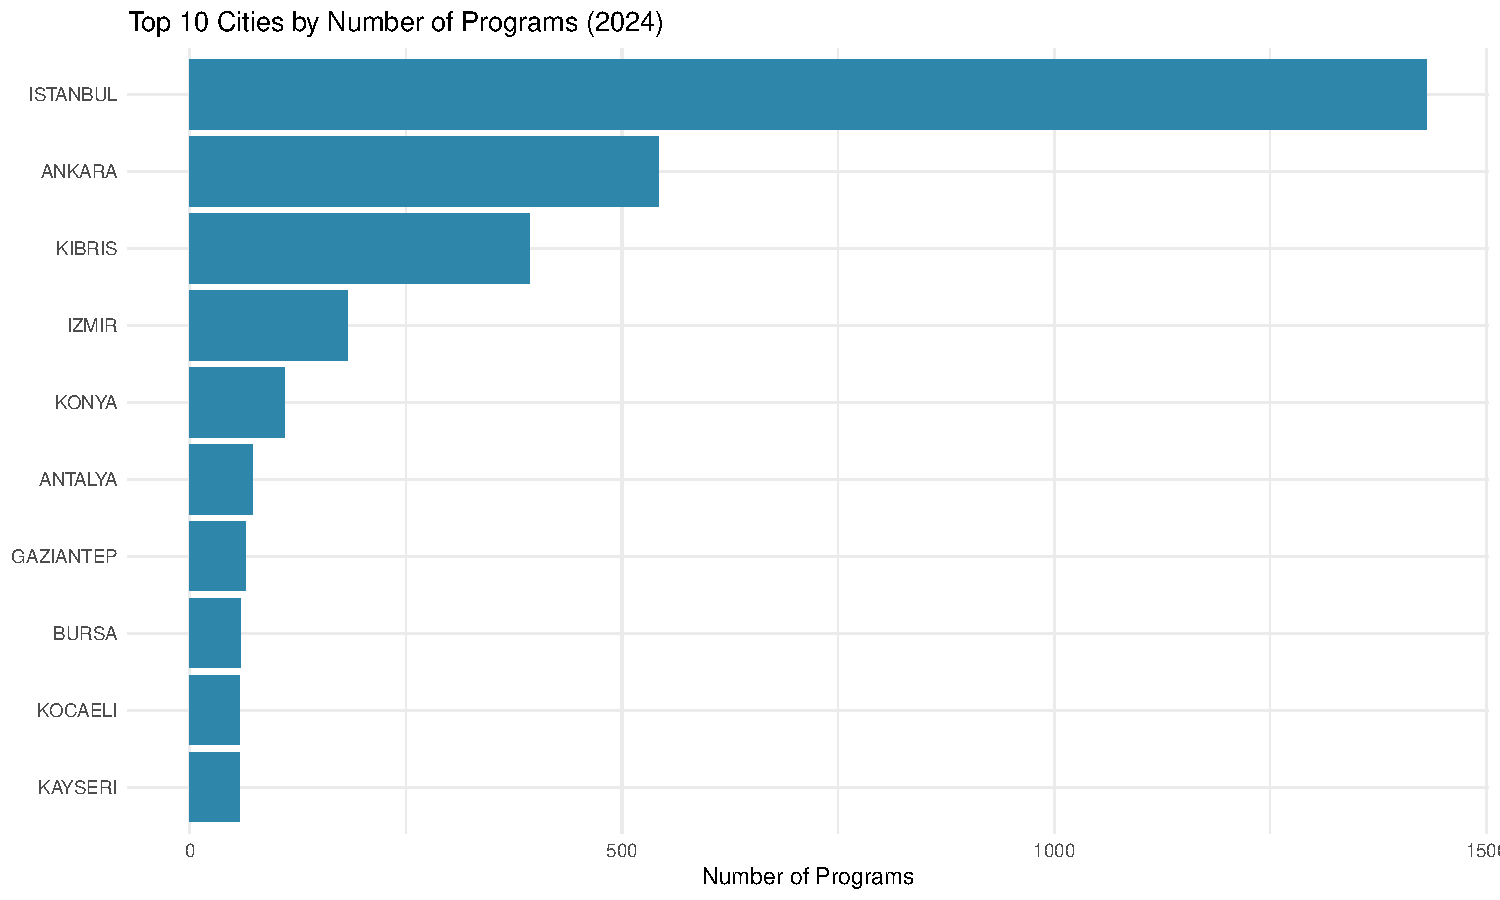
\includegraphics[keepaspectratio]{project_files/figure-pdf/fig-regional-top-cities-1.pdf}}

}

\caption{\label{fig-regional-top-cities}Top 10 cities in Turkey by
number of university programs in 2024.}

\end{figure}%

In Figure~\ref{fig-regional-top-cities}, Istanbul leads by a very large
margin with around 1,400 programs. This is more than double Ankara's
roughly 580. What we did not expect was finding Kıbrıs (Northern Cyprus)
in third place with about 390 programs, ahead of İzmir. This reflects
the large number of Turkish-founded universities operating there that
mainly cater to Turkish students. After Konya in fifth place, the
remaining cities (Antalya, Gaziantep, Bursa, and Kayseri) are all
clustered closely together with similar program counts, ranging roughly
between 57 and 72.

\subsection{3.5 Trend Prediction}\label{trend-prediction}

\begin{Shaded}
\begin{Highlighting}[]
\CommentTok{\# Simple linear model for Bilgisayar Muh.}
\NormalTok{bilgisayar }\OtherTok{\textless{}{-}}\NormalTok{ df }\SpecialCharTok{|\textgreater{}}
  \FunctionTok{filter}\NormalTok{(bolum\_grubu }\SpecialCharTok{==} \StringTok{"Bilgisayar Muh."}\NormalTok{) }\SpecialCharTok{|\textgreater{}}
  \FunctionTok{group\_by}\NormalTok{(year) }\SpecialCharTok{|\textgreater{}}
  \FunctionTok{summarise}\NormalTok{(}\AttributeTok{avg\_puan =} \FunctionTok{mean}\NormalTok{(puan, }\AttributeTok{na.rm =} \ConstantTok{TRUE}\NormalTok{))}

\NormalTok{model }\OtherTok{\textless{}{-}} \FunctionTok{lm}\NormalTok{(avg\_puan }\SpecialCharTok{\textasciitilde{}}\NormalTok{ year, }\AttributeTok{data =}\NormalTok{ bilgisayar)}
\FunctionTok{cat}\NormalTok{(}\StringTok{"Linear model summary:}\SpecialCharTok{\textbackslash{}n}\StringTok{"}\NormalTok{)}
\end{Highlighting}
\end{Shaded}

\begin{verbatim}
Linear model summary:
\end{verbatim}

\begin{Shaded}
\begin{Highlighting}[]
\FunctionTok{cat}\NormalTok{(}\StringTok{"  Coefficient (yearly change):"}\NormalTok{, }\FunctionTok{round}\NormalTok{(}\FunctionTok{coef}\NormalTok{(model)[}\DecValTok{2}\NormalTok{], }\DecValTok{2}\NormalTok{), }\StringTok{"}\SpecialCharTok{\textbackslash{}n}\StringTok{"}\NormalTok{)}
\end{Highlighting}
\end{Shaded}

\begin{verbatim}
  Coefficient (yearly change): -3.38 
\end{verbatim}

\begin{Shaded}
\begin{Highlighting}[]
\FunctionTok{cat}\NormalTok{(}\StringTok{"  R{-}squared:"}\NormalTok{, }\FunctionTok{round}\NormalTok{(}\FunctionTok{summary}\NormalTok{(model)}\SpecialCharTok{$}\NormalTok{r.squared, }\DecValTok{3}\NormalTok{), }\StringTok{"}\SpecialCharTok{\textbackslash{}n}\StringTok{"}\NormalTok{)}
\end{Highlighting}
\end{Shaded}

\begin{verbatim}
  R-squared: 0.028 
\end{verbatim}

\begin{Shaded}
\begin{Highlighting}[]
\CommentTok{\# Predict 2026}
\NormalTok{pred\_2026 }\OtherTok{\textless{}{-}} \FunctionTok{predict}\NormalTok{(model, }\AttributeTok{newdata =} \FunctionTok{data.frame}\NormalTok{(}\AttributeTok{year =} \DecValTok{2026}\NormalTok{))}
\FunctionTok{cat}\NormalTok{(}\StringTok{"  Predicted 2026 avg score:"}\NormalTok{, }\FunctionTok{round}\NormalTok{(pred\_2026, }\DecValTok{1}\NormalTok{), }\StringTok{"}\SpecialCharTok{\textbackslash{}n}\StringTok{"}\NormalTok{)}
\end{Highlighting}
\end{Shaded}

\begin{verbatim}
  Predicted 2026 avg score: 332.6 
\end{verbatim}

\begin{Shaded}
\begin{Highlighting}[]
\FunctionTok{ggplot}\NormalTok{(bilgisayar, }\FunctionTok{aes}\NormalTok{(}\AttributeTok{x =}\NormalTok{ year, }\AttributeTok{y =}\NormalTok{ avg\_puan)) }\SpecialCharTok{+}
  \FunctionTok{geom\_point}\NormalTok{(}\AttributeTok{size =} \DecValTok{3}\NormalTok{, }\AttributeTok{color =} \StringTok{"\#2E86AB"}\NormalTok{) }\SpecialCharTok{+}
  \FunctionTok{geom\_smooth}\NormalTok{(}\AttributeTok{method =} \StringTok{"lm"}\NormalTok{, }\AttributeTok{se =} \ConstantTok{TRUE}\NormalTok{, }\AttributeTok{color =} \StringTok{"\#E74C3C"}\NormalTok{, }\AttributeTok{linetype =} \StringTok{"dashed"}\NormalTok{) }\SpecialCharTok{+}
  \FunctionTok{scale\_x\_continuous}\NormalTok{(}\AttributeTok{breaks =} \DecValTok{2018}\SpecialCharTok{:}\DecValTok{2026}\NormalTok{, }\AttributeTok{limits =} \FunctionTok{c}\NormalTok{(}\DecValTok{2018}\NormalTok{, }\DecValTok{2026}\NormalTok{)) }\SpecialCharTok{+}
  \FunctionTok{labs}\NormalTok{(}\AttributeTok{title =} \StringTok{"Computer Engineering: Score Trend with Linear Prediction"}\NormalTok{,}
       \AttributeTok{x =} \StringTok{"Year"}\NormalTok{, }\AttributeTok{y =} \StringTok{"Average Min Score"}\NormalTok{,}
       \AttributeTok{subtitle =} \FunctionTok{paste0}\NormalTok{(}\StringTok{"Predicted 2026 score: "}\NormalTok{, }\FunctionTok{round}\NormalTok{(pred\_2026, }\DecValTok{1}\NormalTok{))) }\SpecialCharTok{+}
  \FunctionTok{theme\_minimal}\NormalTok{()}
\end{Highlighting}
\end{Shaded}

\begin{verbatim}
`geom_smooth()` using formula = 'y ~ x'
\end{verbatim}

\begin{figure}[H]

\centering{

\pandocbounded{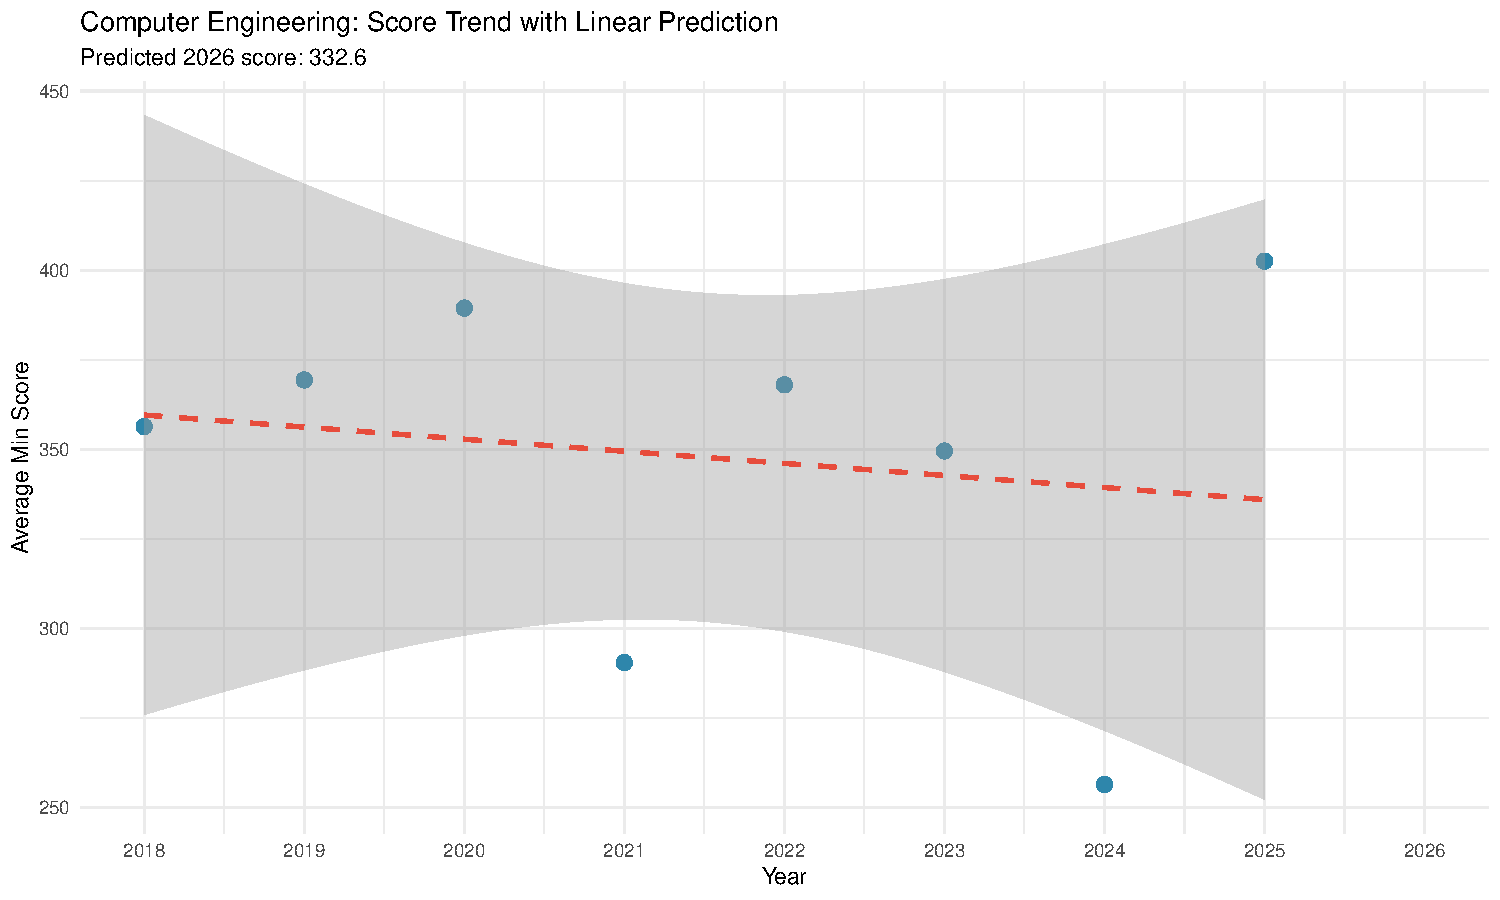
\includegraphics[keepaspectratio]{project_files/figure-pdf/fig-trend-prediction-1.pdf}}

}

\caption{\label{fig-trend-prediction}Linear trend model fitted to
computer engineering average admission scores, with prediction for
2026.}

\end{figure}%

The linear model fitted to computer engineering scores in
Figure~\ref{fig-trend-prediction} shows a slightly negative slope. This
means the trend line is gently declining over the 2018-2025 period. The
decline is mostly driven by the 2021 outlier and the low 2024 value,
which pull the regression line down despite the strong recovery in 2025.
The predicted 2026 score of 332.6 is therefore lower than the most
recent observed value of around 405. This suggests that the model is not
capturing the actual recent momentum well. The confidence interval is
also very wide, which shows high uncertainty. This analysis is a useful
exercise in trend modeling, but a more robust approach (for example,
excluding the anomalous 2021 data point or using a nonlinear model)
would give a more reliable forecast.

\section{4. Discussion}\label{discussion}

The results give us a broad picture of how university preferences have
shifted in Turkey over the last eight years. Medicine and
dentistry/pharmacy remained the most selective fields, which is
consistent with the well-known prestige of healthcare careers in Turkey.
Engineering, despite being the largest category, did not show a clear
directional trend at the aggregate level. The real story for engineering
only appears when we break it down by sub-field. Computer engineering
and software engineering have pulled ahead, while civil engineering has
lost ground. This matches the wider economic story: a growing tech
sector and a slowdown in construction.

There are several limitations in this work that we want to mention.
First, the 2021 data came from a third-party source and shows a clear
discontinuity in our trend charts. We tried to keep this in mind during
interpretation, but it still affects the regression model results.
Second, our keyword-based program name mapping handled most cases well,
but some edge cases (such as rare or newly opened sub-fields) might have
been classified into the ``Diger Muhendislik'' group instead of their
proper category. Third, our linear trend model is intentionally simple,
which is fine as an introductory forecast but is not strong enough to
make policy recommendations. Future work could use ARIMA or other
time-series models that better handle outliers and short series.

Another point worth mentioning is the unexpected finding about Kıbrıs in
the regional analysis. Although it is not officially part of Turkey, the
large number of programs hosted by Turkish-affiliated universities there
is significant. A separate analysis focused only on the Kıbrıs programs
could be an interesting extension of this study.

\section{5. Key Takeaways}\label{key-takeaways}

\begin{itemize}
\tightlist
\item
  This study analyzed university admission trends in Turkey across seven
  field categories using YÖK Atlas data spanning 2018 to 2025. The
  dataset covers tens of thousands of program records from both state
  and private institutions.
\item
  Medicine and dentistry/pharmacy consistently maintained the highest
  admission scores throughout the period. Engineering, despite being the
  largest category by program count, showed a wide internal spread
  driven by the mix of highly selective and open-access programs.
\item
  Computer engineering and software engineering emerged as the most
  competitive engineering sub-fields by 2025. Civil engineering stayed
  at the lower end, which reflects a broader shift in student
  preferences toward technology-oriented careers.
\item
  State and private university engineering programs showed more similar
  score distributions than expected. The key difference is that private
  institutions include a longer tail of very low-scoring programs,
  rather than a uniformly lower performance level.
\item
  A simple linear model predicts a 2026 computer engineering score of
  332.6, but the wide confidence interval and the influence of the
  anomalous 2021 data point make this estimate unreliable. The actual
  2025 value of around 405 suggests the real trend may be stronger than
  the model captures.
\end{itemize}

\section{6. Conclusion}\label{conclusion}

This project tracked how Turkish university preferences have evolved
across seven major field categories between 2018 and 2025. Combining
three different data sources allowed us to build a continuous picture
across the years, even though it introduced some methodological
challenges. The clearest signals from the data are the steady dominance
of medicine and dentistry, the rise of computer-related engineering
fields, and the relative decline of civil engineering. These findings
are consistent with broader economic and labor market trends in Turkey.
We hope this work provides a useful starting point for further analyses,
especially ones that incorporate additional dimensions such as
employment outcomes or program-specific student demographics.

\section{References}\label{references}

\begin{itemize}
\tightlist
\item
  YÖK Atlas. Council of Higher Education, Turkey.
  \url{https://yokatlas.yok.gov.tr/}
\item
  Cavus, M., \& Aydin, O. \emph{thestats: An R package for YÖK Atlas
  data.} \url{https://github.com/analyticsresearchlab/thestats}
\item
  MorphaxTheDeveloper. \emph{YÖK Atlas 2025 Dataset.}
  \url{https://github.com/MorphaxTheDeveloper/yokatlas-dataset-2025}
\end{itemize}

\emph{AI usage note: Claude was used to assist with data collection
scripting, preprocessing of multiple data sources and code debugging.
All analysis interpretations and written content belongs to the
authors.}




\end{document}
